\section{Taratura di un trasduttore di pressione}
Il trasduttore di pressione è un componente della catena di misura preposto a quantificare il valore della pressione da misurare sfruttando un principio fisico.\\\\
La pressione misurata può essere riferita al vuoto (nel caso di trasduttori assoluti) oppure rispetto ad una pressione di riferimento (nel caso di trasduttori differenziali).\\\\
L'obiettivo del presente esperimento è la taratura di un trasduttore differenziale capacitivo bidirezionale ad alta precisione, il SETRA mod. 239 C.
\begin{figure}[h]
    \centering
    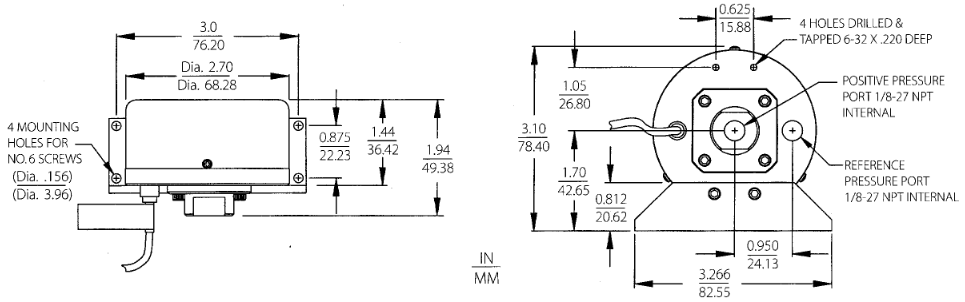
\includegraphics[width=\linewidth]{images//1/setra.png}
    \caption{Trasduttore di pressione SETRA mod. 239 C}
\end{figure}

\subsection{Descrizione dell'esperimento}
I trasduttori differenziali misurano una differenza di pressione $p-p_{rif}$ e presentano pertanto due ingressi, uno per la pressione da misurare ed uno per la pressione di riferimento. La pressione di riferimento viene definita dall'operatore a seconda della misura da effettuare. Nel caso in esame, questa è la pressione statica della corrente nel cuore potenziale di un getto.\\\\
Nei trasduttori capacitivi viene sfruttata la variazione di capacità di un condensatore sotto l'effetto della forza di pressione. Una faccia del condensatore è fissa mentre l'altra è flessibile e per effetto dell'azione di pressione agente su di essa si deforma variando la distanza tra le due facce e quindi la capacità.\\\\
Alla variazione della capacità $C(t)$ è legata la variazione del segnale elettrico in uscita, che tipicamente è una tensione $E(t)$. La capacità di un condensatore è definita dalla seguente relazione:
\begin{equation*}
    C = \frac{K_d A}{X_0}
\end{equation*}
in cui $K_d$ è la costante dielettrica della capacità, $A$ è la superficie della parete e $X_0$ è la distanza tra le facce del condensatore. Per effetto della deformazione, varia la distanza $X_0$ tra la membrana flessibile e la parte fissa. Ad una variazione della capacità $\Delta C$ corrisponde pertanto una variazione di potenziale ai capi del condensatore:
\begin{equation*}
    \Delta V = \frac{\Delta C}{C}E_a
\end{equation*}
dove $\Delta C/C$ è la variazione della capacità dovuta alla pressione mentre $E_a$ è la tensione di alimentazione del condensatore. Risulta pertanto $\Delta V = f(\Delta p)$.\\\\
Il legame tra la differenza di pressione $\Delta p$ e la differenza di tensione $\Delta V$ prende il nome di curva di taratura del trasduttore. Il segnale elettrico e la pressione applicata sono correlate attraverso una costante di taratura $K_t$ che va determinata sperimentalmente.\\\\
Eseguire la taratura del trasduttore significa quindi determinare il valore della costante di taratura $K_t$.

\subsection{Catena di misura}
Per effettuare la taratura del trasduttore, e quindi trovare una relazione che associa ad ogni valore di tensione in uscita un valore di differenza di pressione applicata, è necessario conoscere l'entità di tale pressione. Si utilizza quindi un flusso noto: il cuore potenziale di un getto.
\begin{figure}[H]
    \centering
    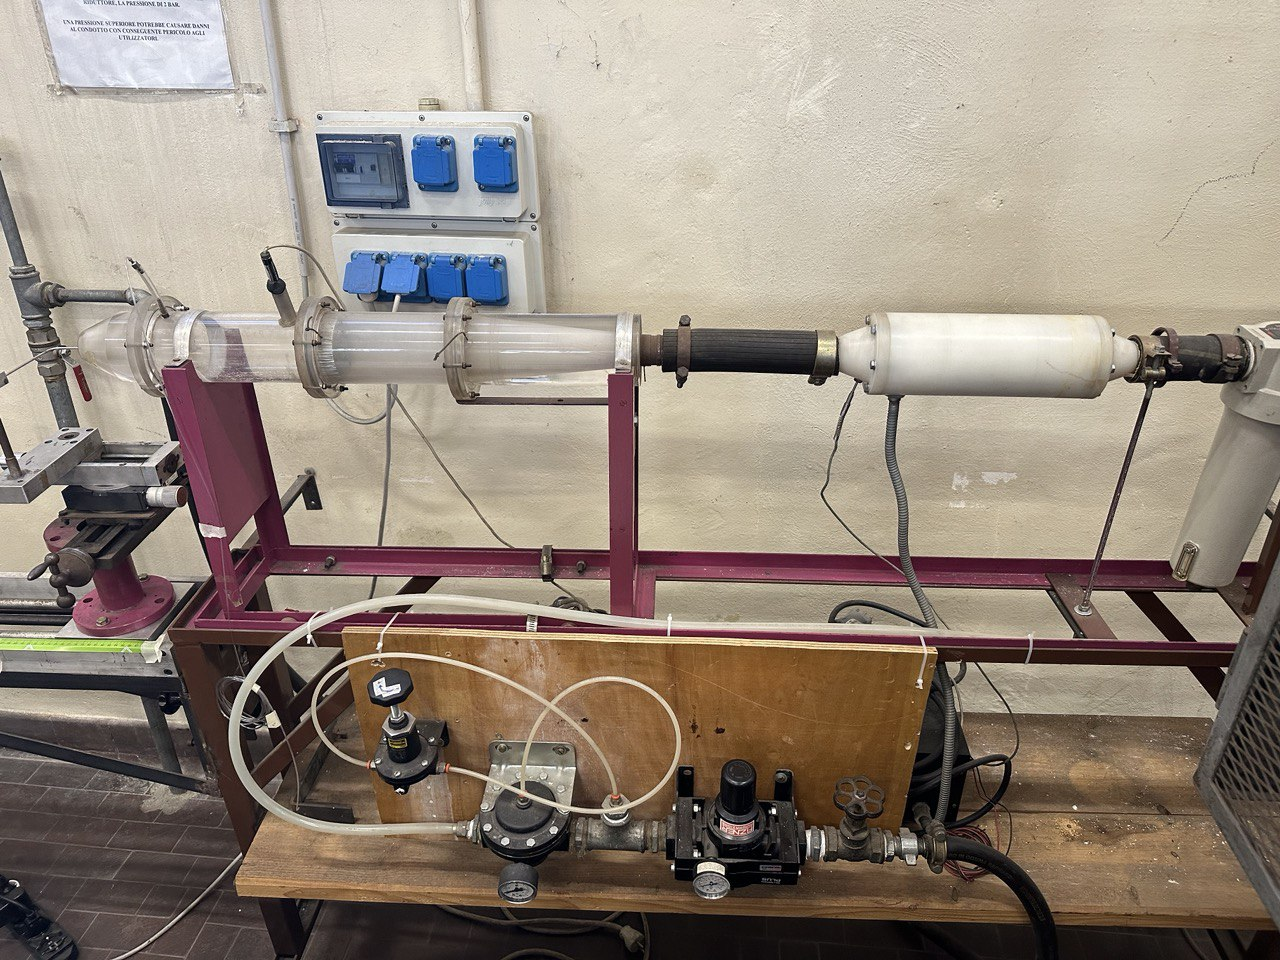
\includegraphics[width=.8\textwidth]{images/1/getto.jpg}
    \caption{Sistema di regolazione della portata del getto}
\end{figure}

\noindent Per rilevare la pressione totale e la pressione statica nel cuore potenziale del getto è utilizzato un tubo di Pitot.
\begin{figure}[H]
    \centering
    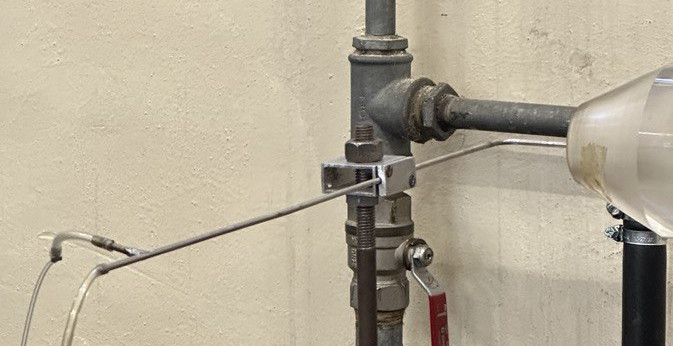
\includegraphics[width=.45\textwidth]{images/1/pitot.jpg}
    \caption{Tubo di pitot nel cuore potenziale del getto}
\end{figure}

\noindent Per ricavare il corretto valore di differenza di pressione dal tubo di Pitot si utilizza il manometro di Betz, uno strumento di grande precisione costituito da un serbatoio di acqua distillata entro cui è presente una scala graduata galleggiante. La differenza di pressione tra due camere entro cui è contenuto il liquido produce uno spostamento verticale del galleggiante.
\begin{figure}[h]
    \centering
    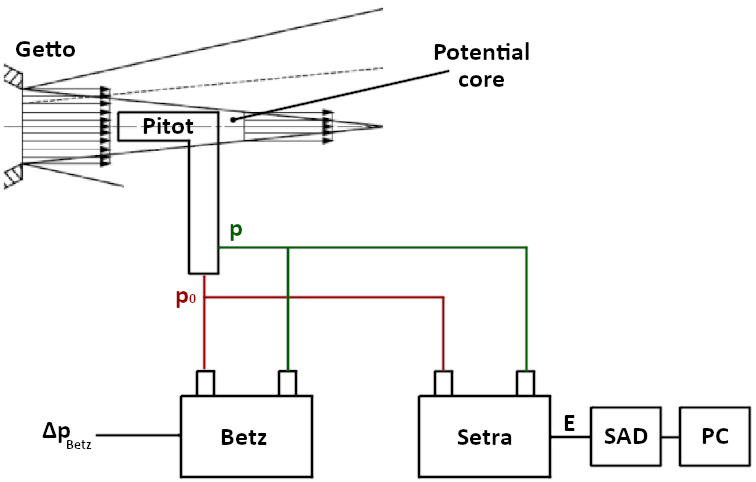
\includegraphics[width=.7\textwidth]{images/1/catena.png}
    \caption{Catena di misura}
\end{figure}

\noindent La catena di misura è quindi composta da:
\begin{itemize}
    \item Getto;
    \item Tubo di Pitot, posizionato nel cuore potenziale del getto;
    \item Trasduttore di pressione SETRA mod. 239 C; 
    \item Manometro di Betz;
    \item Sistema di acquisizione dati (SAD) e PC con LabView.
\end{itemize}

\noindent I canali pneumatici di pressione statica e pressione totale rilevate dal tubo di Pitot sono connessi sia al manometro di Betz che al trasduttore di pressione SETRA mod 239 C. Pertanto, tramite il sistema di acquisizione dati, è possibile registrare il valore di tensione in uscita ed associarlo alla relativa differenza di pressione indicata dal manometro di Betz.\\\\

\subsection{Procedura sperimentale}
Come prima operazione è necessario misurare la tensione di offset $E_0$, cioè la tensione in uscita al trasduttore quando non è applicata alcuna differenza di pressione. Per fare ciò, si acquisiscono i dati in uscita al trasduttore con il getto spento. Si ottiene la seguente tensione di offset:
\begin{equation*}
    E_0 = -8.57\cdot 10^{-4}\ V
\end{equation*}
Una volta misurata tale tensione, si può scomporre il segnale in uscita come:
\begin{equation*}
    E(\Delta p) = E_0 + \Delta E(\Delta p)
\end{equation*}
Si procede variando la portata e quindi la pressione dinamica nel cuore potenziale del getto ed acquisendo per ogni valore di differenza di pressione indicato sul manometro di Betz il valore di tensione in uscita corrispondente.\\\\
Il manometro di Betz è caratterizzato da una bassa risposta in frequenza, pertanto per ogni variazione di portata del getto è necessario attendere almeno 30 secondi per fare in modo che il manometro di Betz riporti il valore di differenza di pressione corretto sulla scala graduata.\\\\
I dati sono acquisiti con una frequenza $f_s=2$ kHz per un periodo di $T=1$ s.\\\\
I dati grezzi acquisiti durante la procedura sono riportati in appendice \ref{a1}.\\\\

\subsection{Analisi dati e costante di taratura}
L'analisi dati è condotta con l'ausilio di un codice Python, riportato in appendice \ref{b1}.\\\\
La relazione che lega la differenza di pressione applicata, misurata con il manometro di Betz, e il segnale di tensione in uscita dal trasduttore di pressione è la seguente:
\begin{equation*}
    \Delta p_{Betz} = K_t \Delta E = K_t (E - E_0)
\end{equation*}
Da cui si ricava:
\begin{equation*}
    K_t = \frac{\Delta p_{Betz}}{\Delta E}
\end{equation*}
\newpage
\noindent I dati sperimentali acquisiti, con le relative barre di errore, sono riportati nel seguente diagramma:
\begin{figure}[h]
    \centering
    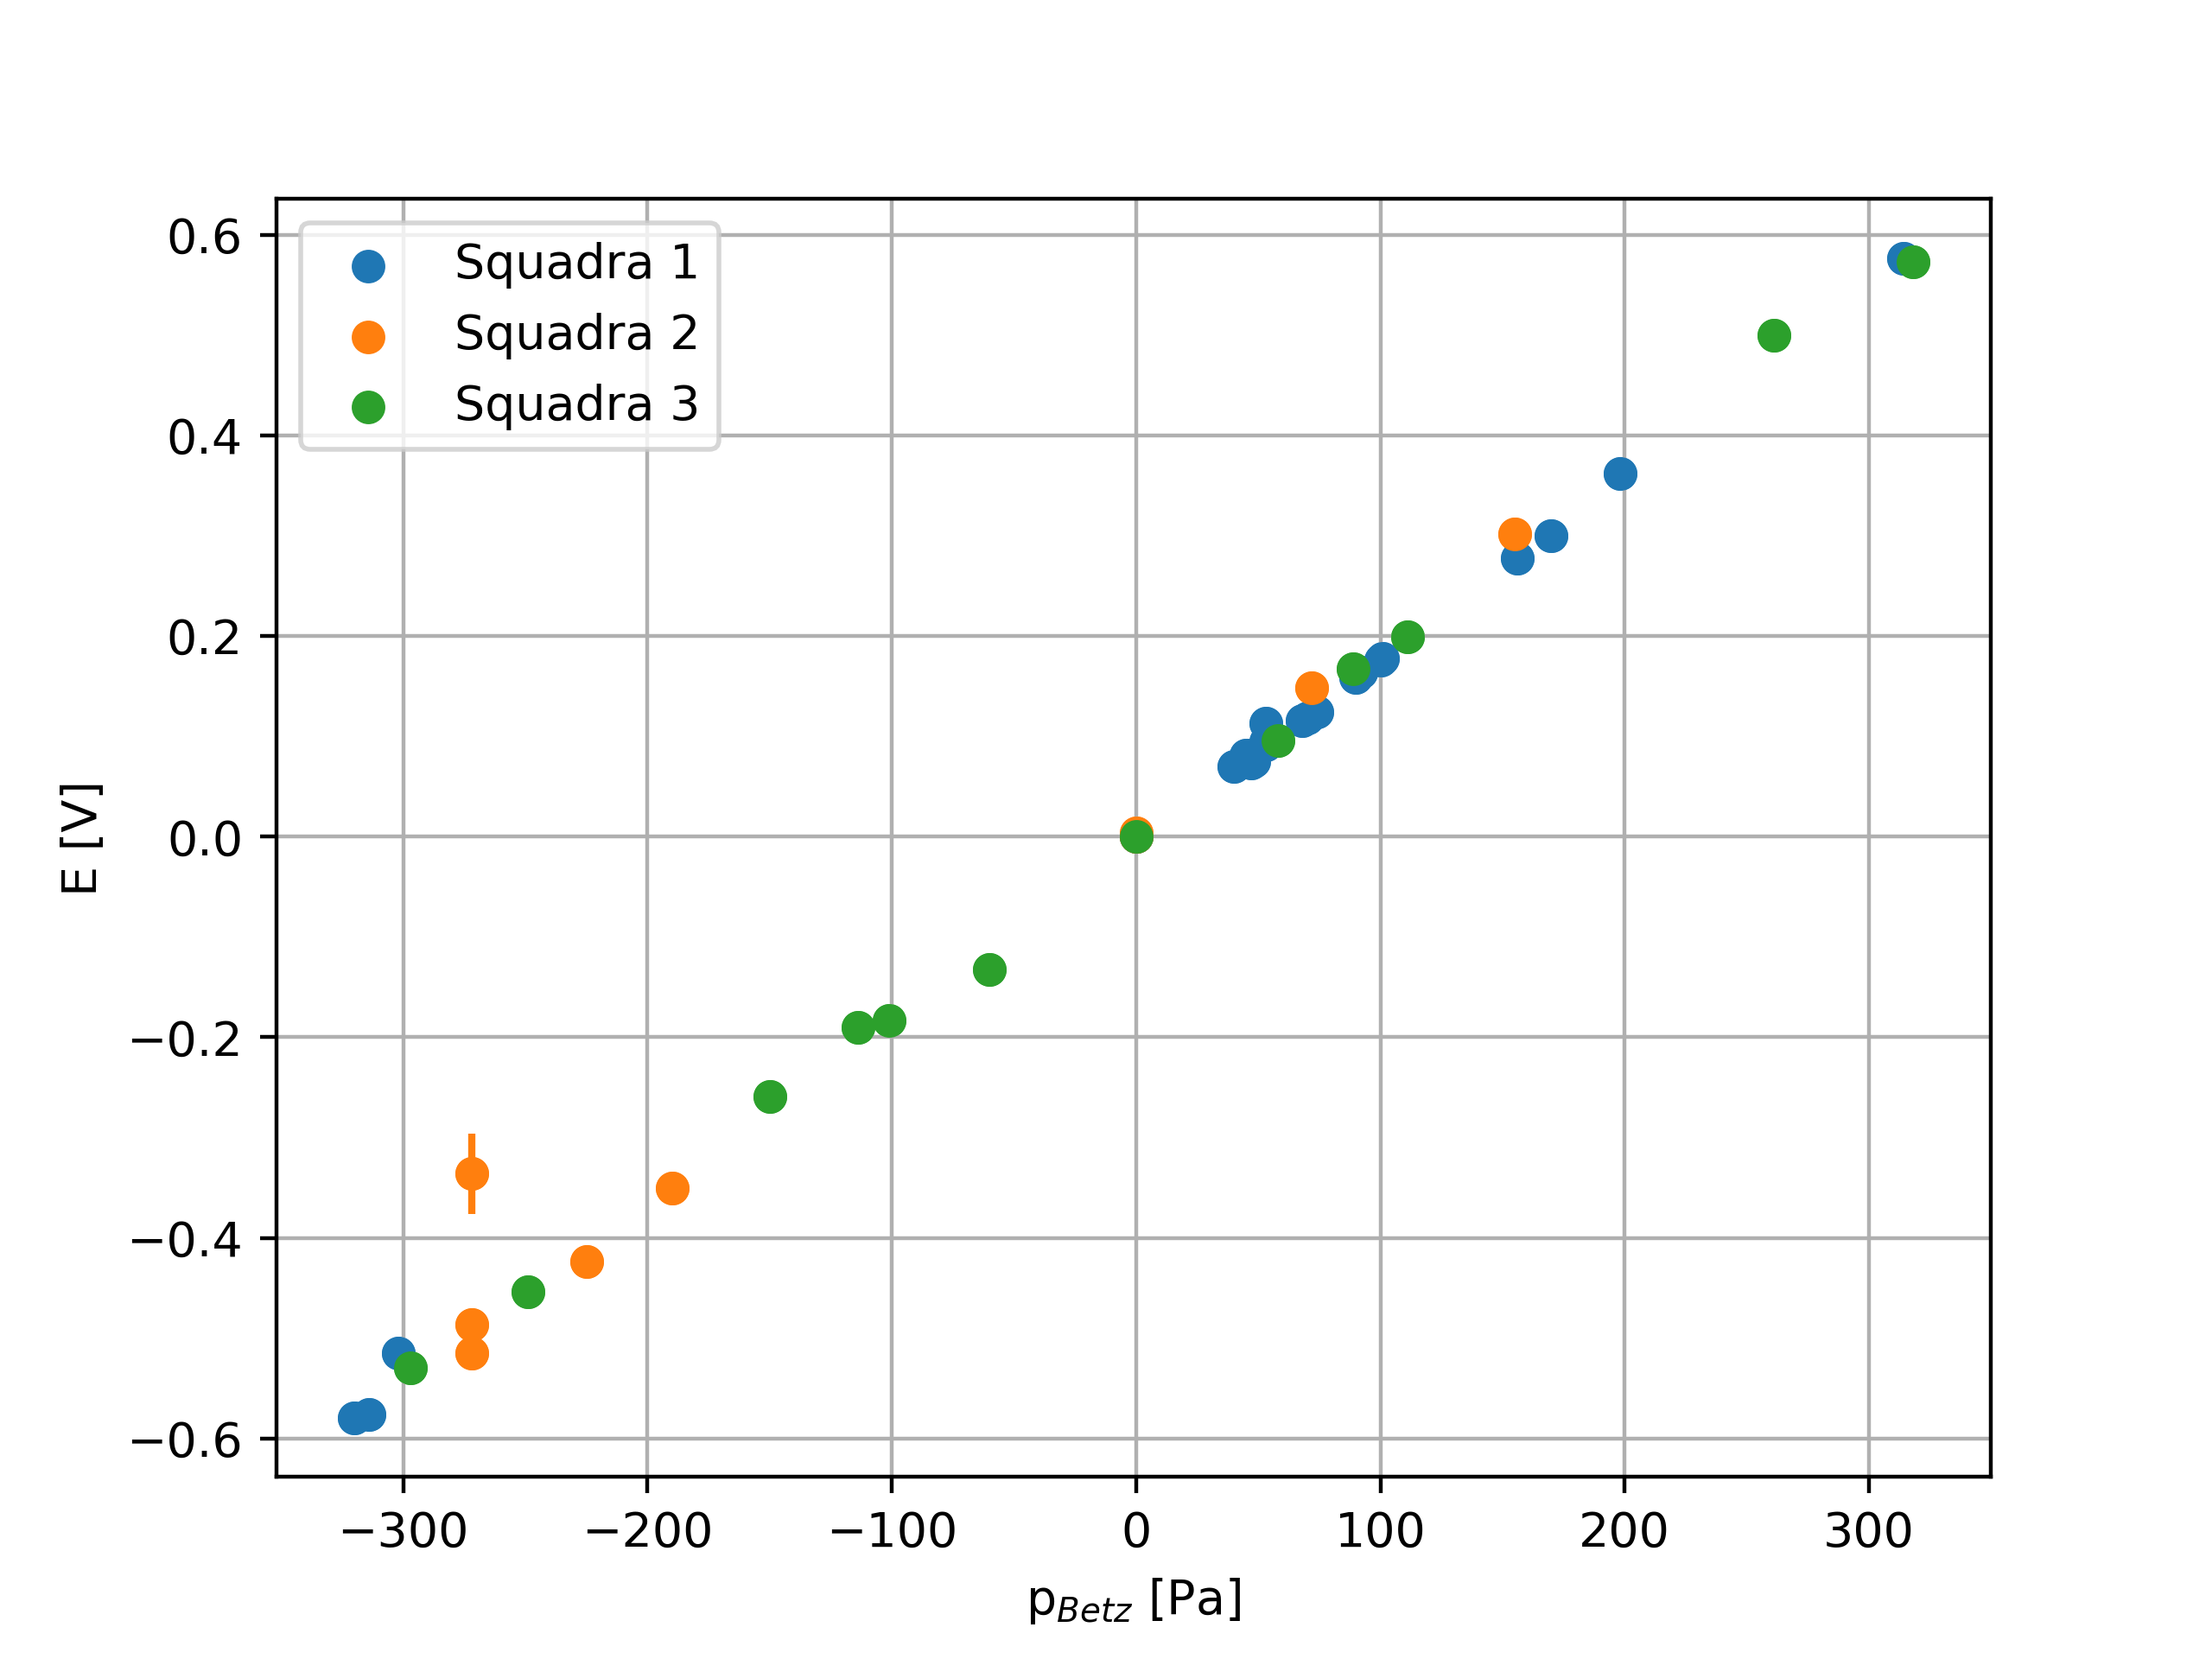
\includegraphics[width=\textwidth]{images/1/kt.png}
    \caption{Dati sperimentali}
\end{figure}

\noindent Attraverso una semplice interpolazione lineare dei dati, è possibile ricavare il valore sperimentale della costante di taratura per le tre squadre:

\begin{equation*}
    \text{Squadra 1: } K_t = 556.69\ \text{Pa/V}
\end{equation*}
\begin{equation*}
    \text{Squadra 2: } K_t = 549.38\ \text{Pa/V}
\end{equation*}
\begin{equation*}
    \text{Squadra 3: } K_t = 549.47\ \text{Pa/V}
\end{equation*}
Per semplicità, nelle seguenti esercitazioni la costante di taratura è imposta pari a
\begin{equation*}
    K_t = 550\ \text{Pa/V}
\end{equation*}

\newpage
\subsection{Tempo caratteristico}
Poiché il manometro di Betz è caratterizzato da una lenta risposta in frequenza, è opportuno indagare il fenomeno transitorio della linea pneumatica ed il relativo tempo caratteristico $\tau$.\\\\
Per fare ciò, sono acquisite le tensioni di uscita dal trasduttore con una frequenza di campionamento $f_{samp}=2000$ Hz per un periodo $T$ di 2 minuti.\\\\
Per determinare il tempo caratteristico si interpolano i dati sperimentali con una curva esponenziale, del tipo:
\begin{equation*}
    E(t) = Ae^{bt} = Ae^{-\frac t\tau}
\end{equation*}
Maneggiando tale relazione, si ottiene:
\begin{equation*}
    \log E(t) = \log A + bt = c_1 t + c_2 \quad \Rightarrow \quad b = -\frac1\tau = c_1 \ ; \ A = e^{c_2}
\end{equation*}
Si ricava dunque il tempo caratteristico della linea pneumatica:
\begin{equation*}
    \tau = 295.06 \text{s}
\end{equation*}
Il valore ottenuto risulta coerente con la risposta in frequenza del manometro di Betz.
\begin{figure}[h!]
    \centering
    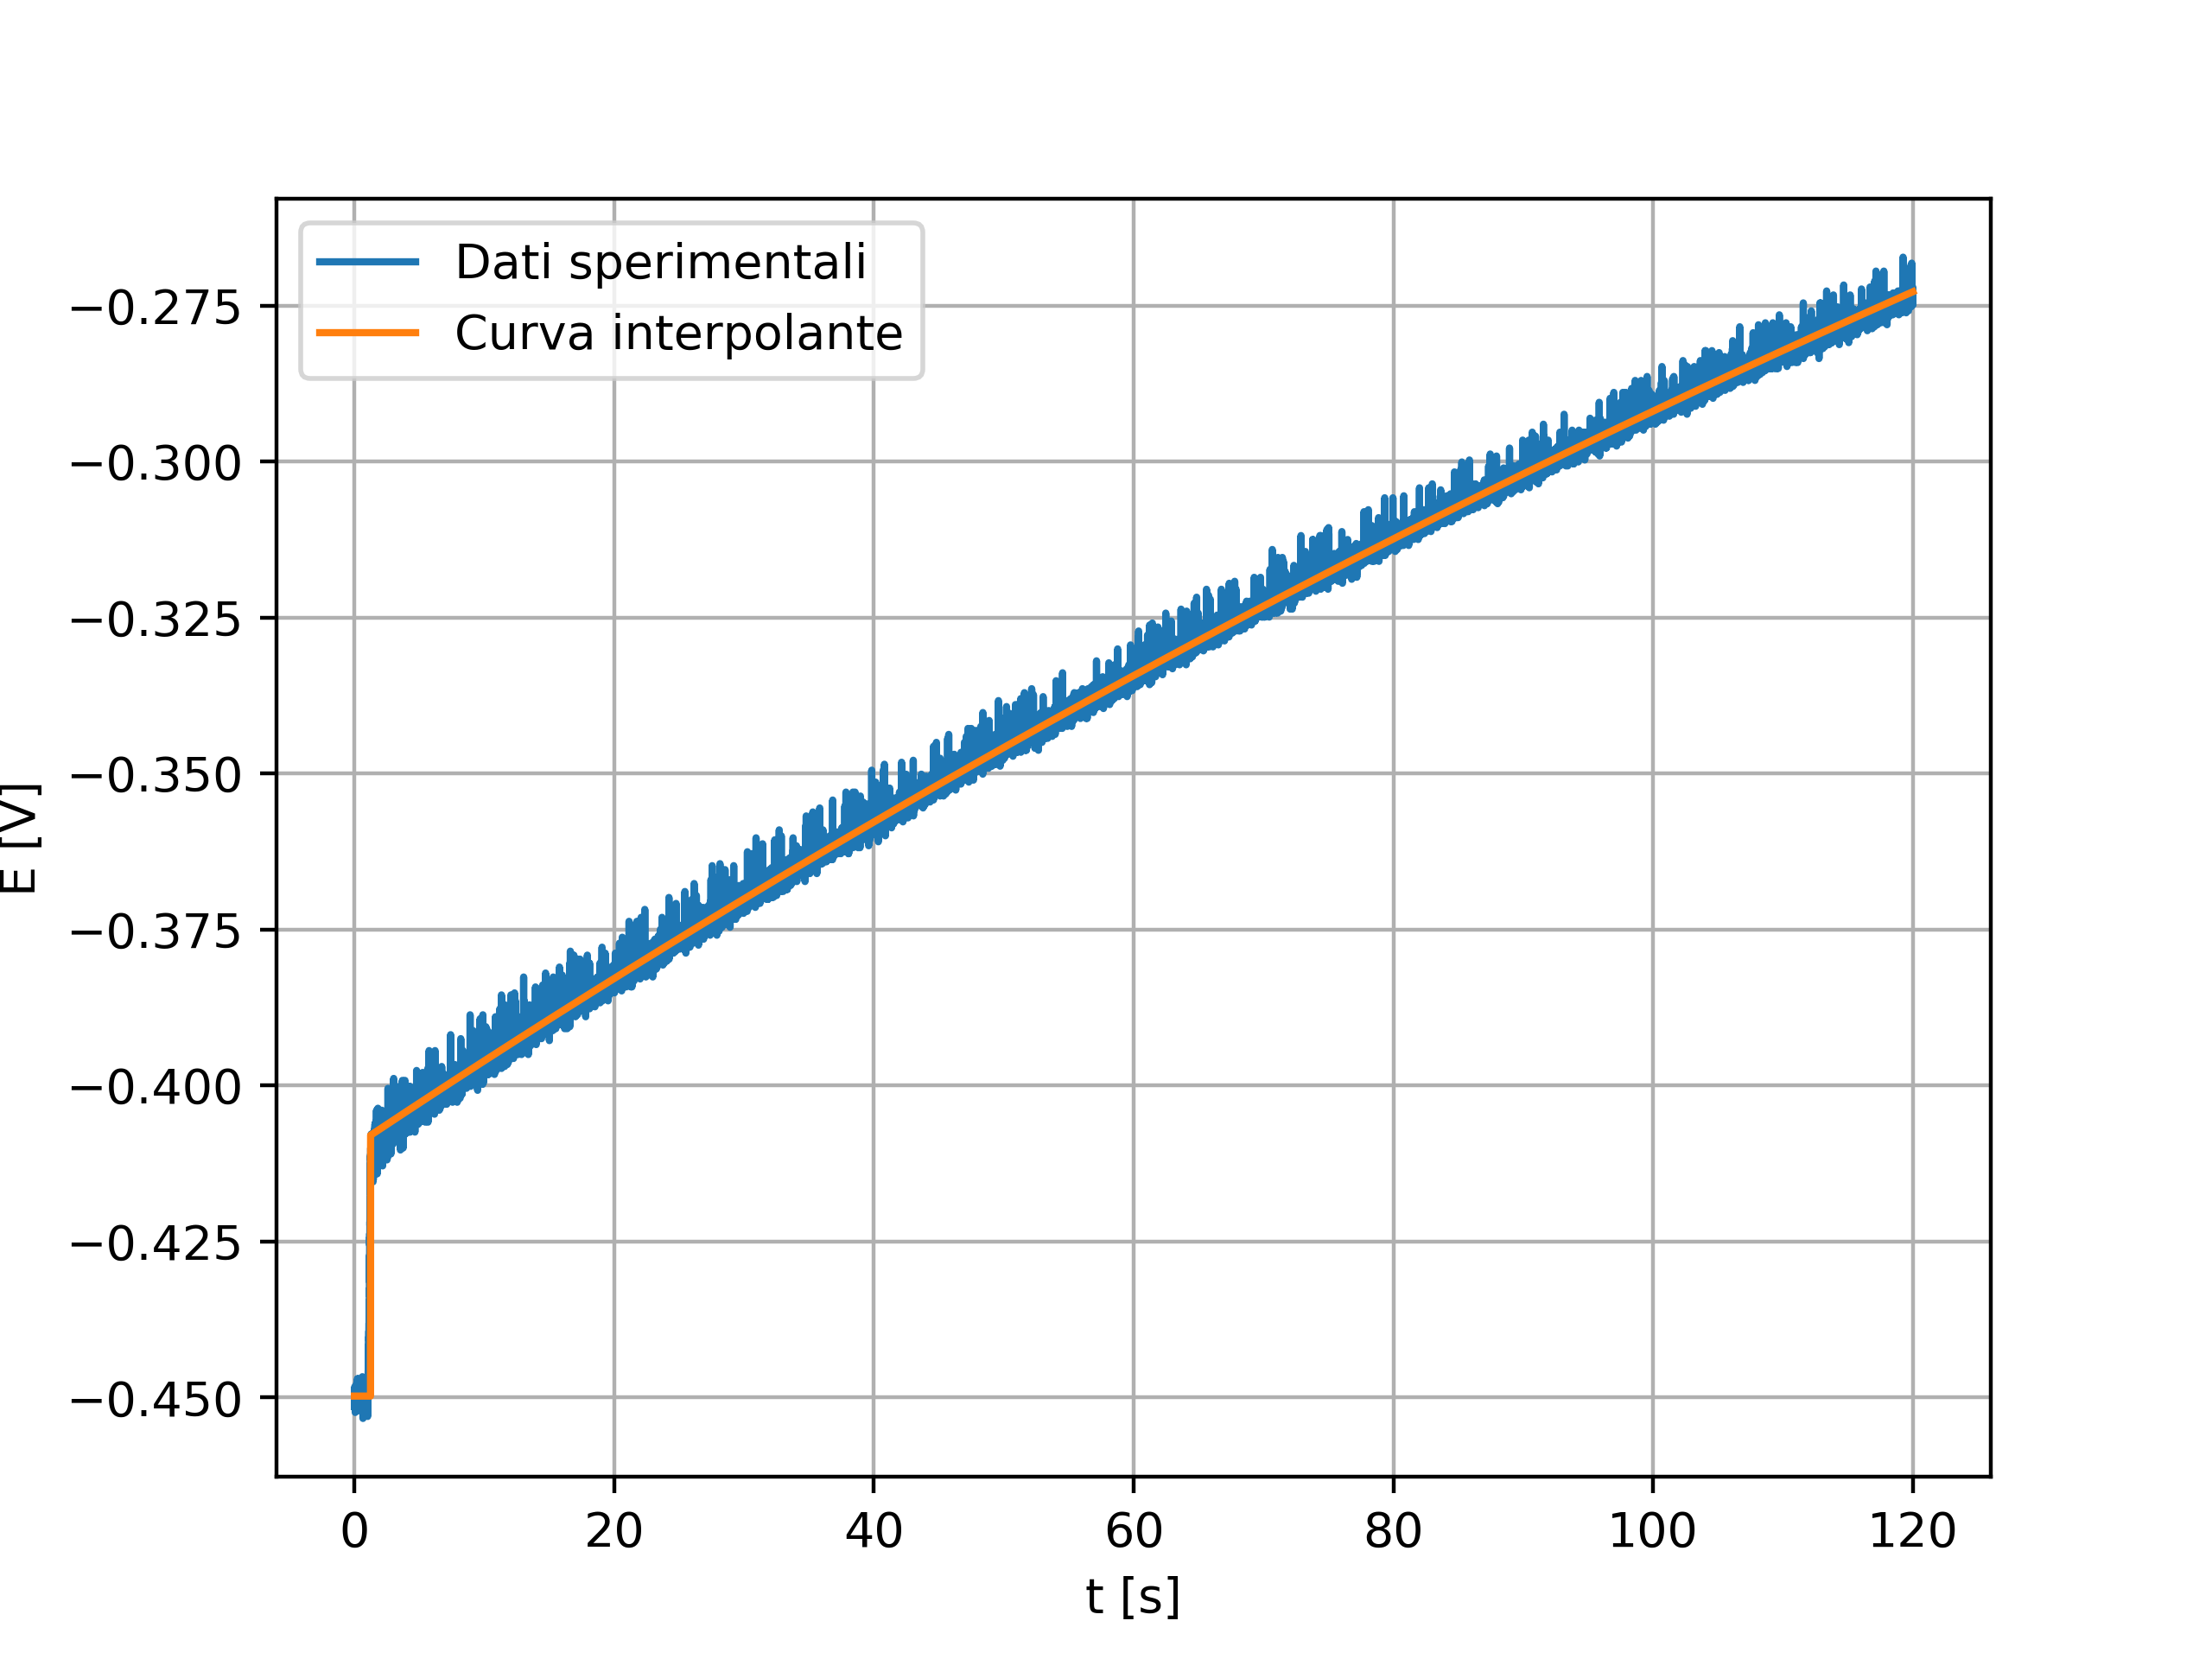
\includegraphics[width=.8\textwidth]{images/1/transitorio.png}
    \caption{Transitorio}\label{fig:t1}
\end{figure}